\begin{surferPage}[Cono cuadrático]{Cono cuadrático}
Se dice que una superficie es \emph{no singular} o \emph{lisa}
si no tiene, en sentido intuitivo, puntas, aristas o pliegues
(a los cuales se llama \emph{singularidades}).
    \vspace{-0.2cm}
    \begin{center}
      \begin{tabular}{@{}c@{}c@{}c@{}c@{}}
        \begin{tabular}{@{}c}
          \includegraphics[width=1.1cm]{../../common/images/kugel}
        \end{tabular}
        &
        \begin{tabular}{@{}c}
          \includegraphics[width=1.1cm]{../../common/images/torus}
        \end{tabular}
        &
        \begin{tabular}{c@{}}
          \includegraphics[width=1.1cm]{../../common/images/kegel}
        \end{tabular}
        &
        \begin{tabular}{c@{}}
          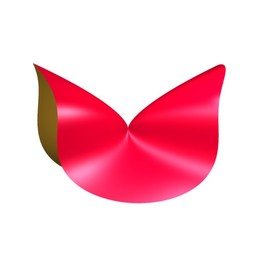
\includegraphics[width=1.1cm]{../../common/images/A2pm_ill}
        \end{tabular}
      \end{tabular}
    \end{center}
    \vspace*{-0.4em}
La esfera o el toro son lisas. El cono cuadrático tiene un punto singular
del tipo más simple ($A_1^{+-}$). Si se `deforma' su ecuación
$x^2+y^2-z^2=0$ poniendo en lugar del 0 un número $a$ cualquiera,
la superficie
\[x^2+y^2-z^2=a\]
es lisa si $a\neq0$. Imágenes para $a=-\frac12$, $a=0$, $a=\frac12$:
    %
    \begin{center}
      \begin{tabular}{@{}c@{\quad}c@{\quad}c@{}}
        \begin{tabular}{@{}c@{}}
          \includegraphics[width=1.2cm]{../../common/images/A1pm_0}
        \end{tabular}
        &
        \begin{tabular}{@{}c@{}}
          \includegraphics[width=1.2cm]{../../common/images/A1pm_1}
        \end{tabular}
        &
        \begin{tabular}{@{}c@{}}
          \includegraphics[width=1.2cm]{../../common/images/A1pm_2}
        \end{tabular}
      \end{tabular}
    \end{center}
    \vspace*{-0.4em}
En los ejemplos que siguen se verá que es posible deformar singularidades
más complicadas de manera que aparezcan varias singularidades como las
del cono cuadrático (singularidades cónicas).
 
\end{surferPage}
